\section{Introduction}

According to research by First Education (2022), the Dutch are positioned as the most proficient English-speaking population globally. Other countries that achieved a position in the top 10 ranking were Denmark, Belgium, Sweden, Finland, and Germany. While a proud Dutchman may attribute this success to hard work and dedication, it is worth considering other factors that could be at play here. Notably, these countries with commendable English proficiency are all located in North Europe and speak very similar languages.  

Linguistics offers a unique perspective on the relationships between different languages. By comparing the vocabulary, grammar and sound systems of various languages, researchers have identified related language families and have constructed language family trees to illustrate the evolution and divergence of languages over time. Thanks to that research, we know that many countries with notable position in the English Proficiency Index share a common linguistic background. Such a linguistic background, or language family, thus may provide a foundation for proficiency in a new language. 

This would imply that certain languages are easier to learn for certain population groups. For Atlan, it is deemed important that it will become a language that is easy and quick to learn for \textit{everybody}. This is a challenging task but might be achievable if we find some sort of shared background between almost every natural language. If it is possible to find words that look similar in different languages, which are known as cognates, the translation for those words in Atlan can be designed to resemble them as much as possible. With a model that can do this on a large scale, Atlan will become easy, neutral, and global.  

To achieve this, it is first key to create some understandings of what methods are used to compare different languages. Therefore, we will take a closer look at the so-called cosine similarity. Thereafter, it is necessary to conduct an examination of the existing language families that exist. In that way, we gain a deeper insight into the connections between existing natural languages. In addition, with that gained understanding, it is possible to decide which language we will make available in contributing to the process of cognate finding. The most spoken languages are weighed against each other to create a dataset that is representative of the real world. All these pieces of the puzzle come together in the final part of this chapter, where the computer program that we used to generate words in Atlan will be discussed.

\section{Comparison methods and language families -- {\small Jep Antonisse}}

\subsection{Cosine Similarity}

According to research by First Education (2022), the Dutch are positioned as the most proficient English-speaking population globally. Other countries that achieved a position in the top 10 ranking were Denmark, Belgium, Sweden, Finland, and Germany. While a proud Dutchman may attribute this success to hard work and dedication, it is worth considering other factors that could be at play here. Notably, these countries with commendable English proficiency are all located in North Europe and speak very similar languages.  

Linguistics offers a unique perspective on the relationships between different languages. By comparing the vocabulary, grammar and sound systems of various languages, researchers have identified related language families and have constructed language family trees to illustrate the evolution and divergence of languages over time. Thanks to that research, we know that many countries with notable position in the English Proficiency Index share a common linguistic background. Such a linguistic background, or language family, thus may provide a foundation for proficiency in a new language. 

This would imply that certain languages are easier to learn for certain population groups. For Atlan, it is deemed important that it will become a language that is easy and quick to learn for \textit{everybody}. This is a challenging task but might be achievable if we find some sort of shared background between almost every natural language. If it is possible to find words that look similar in different languages, which are known as cognates, the translation for those words in Atlan can be designed to resemble them as much as possible. With a model that can do this on a large scale, Atlan will become easy, neutral, and global.  

To achieve this, it is first key to create some understandings of what methods are used to compare different languages. Therefore, we will take a closer look at the so-called cosine similarity. Thereafter, it is necessary to conduct an examination of the existing language families that exist. In that way, we gain a deeper insight into the connections between existing natural languages. In addition, with that gained understanding, it is possible to decide which language we will make available in contributing to the process of cognate finding. The most spoken languages are weighed against each other to create a dataset that is representative of the real world. All these pieces of the puzzle come together in the final part of this chapter, where the computer program that we used to generate words in Atlan will be discussed.
\vspace{0.3cm}

\begin{center}
\resizebox{1\textwidth}{!}{
\begin{tabular}{|c|c|c|}
\hline
{\bf Text} & {\bf Frequency \lq\lq Merry"} & {\bf Frequency \lq\lq christmas"} \\
\hline

\lq\lq Merry christmas " & 1 & 1 \\

\lq\lq Christmas" & 0 & 1 \\
\hline
\end{tabular}
	}

{\it \footnotesize Table 6.1: Word-appearance in \lq\lq Merry" and \lq\lq Merry christmas".}
\end{center}
\vspace{0.3cm}

 \noindent This table can be visualized in a two-dimensional array, where on each axis the count of a word is represented. Now both texts can be placed as a dot on this grid accordingly. Drawing two lines from each point to the origin of the grid creates an angle between those lines. This angle at the origin can be calculated, in this case it would be 45$^{\circ}$ . To finish the cosine similarity, all that is needed now is to take the cosine of this angle, in this example \textit{cos (45)} = 0.71. 


%%%%AFBEELDING

If the compared sentences are identical, the two dots would be placed on the same place in the grid. Thus, the lines towards the origin would fall precisely over each other. Therefore, the angle between both lines would be 0$^{\circ}$, resulting in a cosine score of \textit{cos (0) = 1.} On the other hand, if both sentences have not a single element in common, the lines would be perpendicular to each other. With an angle of 90$^{\circ}$, the cosine similarity would return \textit{cos (90) = 0.} Thus, in any case, the cosine similarity gives a score between 0 and 1, showing the degree of similarity. 

As another example, let’s compare two words: \textit{‘Bert’} to \textit{‘Ernie’}. Instead of words, the vector now can be made up of letters. In a table, this would look like this:

\begin{center}
\begin{tabular}{|l|c|c|c|c|c|c|c|}
\hline
{\bf Name} & {\bf E} & {\bf R} & {\bf N} & {\bf I} & {\bf B} & {\bf T} \\
\hline
{\bf Ernie} & 2 & 1 & 1 & 1 & 0 & 0\\
{\bf Bert} & 1 & 1 & 0 & 0  & 1 & 1 \\
\hline
\end{tabular}

{\it \footnotesize Table 6.2: Letter frequency in the words \lq\lq Bert" and \lq\lq Ernie".}
\end{center}

\begin{samepage}
\noindent With six different letters occurring, it would be possible to place both \textit{‘Bert’} and \textit{‘Ernie’} in a six-dimensional grid and draw the lines to the origin. However, it is impossible for humans to visualize a six-dimensional graph. Thus, we need a new way to calculate the angle between the two vectors. Luckily, there exists a formula to compute the cosine similarity. 

\begin{center}
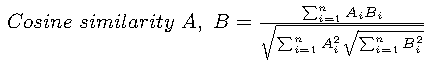
\includepdf[scale=0.5]{./Mainmatter/sum.pdf}
\end{center}
\end{samepage}

%\begin{equation}
%Cosine~ similarity~ A, ~B = \frac{\sum_{i=1}^{n} A_i B_i}{\sqrt{\sum_{i=1}^{n} A_i^2 \sqrt{\sum_{i=1}^{n} B_i^2}}}
%\end{equation}

In less mathematical terms, what this means is that each element of the two vectors A and B are compared. The products of all the elements are then summed up and divided by the length of both the vectors together. If we fill in the numbers for our Bert-Ernie-comparison, it will look like this: 

\begin{equation}
	\frac{1 \times 2 + 1 \times 1 + 1 \times 0 + 1 \times 0 + 0 \times 1 + 1 \times 0}{\sqrt{2^2 + 1^2 + 1^2 + 1^2 + 0^2 + 0^2 \sqrt{1^2 + 1^2 + 0^2 + 0^2 + 1^2 + 1^2}}} = 0.56
\end{equation}

Nevertheless, converting the words based solely on letter frequency inadvertently results in losing vital information about the arrangement of the letters. This preservation is of utmost importance for our project since we try to find patterns and therefore adjacent letter combinations. To address this concern, we introduced a slight adjustment to the regular cosine similarity, where each index with the same character in both words also scores a small point. In this way, our cosine similarity tries to reward words that have the same letters on the same place.

\subsection{Language families}

The use of various comparison methods, similar to the cosine similarity, allowed linguists to identify several groups of related languages. These groups, or language families, were categorized based on common linguistic features and a shared common ancestor (Campbell, 2018). Such a common Proto-Language allows researchers to trace origins of various languages to a single root. However, this does not necessarily need to be the case. There exist languages for which it is impossible to classify them as part of a language family, such as Basque (Campbell, 2010). Researchers speculate that it might be possible that these languages, known as language isolates, might have had related languages in the past, that went instinct unrecorded. Therefore, these languages now form their own language family, with them being the only member. On the other hand, not only genetic proximity between languages is enough to be placed in the same language family. Languages that are constructed instead of naturally developed cannot be considered part of any language family, since they do not have a shared ancestor with any other language (Campbell, 2018). 

Although this means that the total number of language families in the world might be in the hundreds, not all are equally relevant today. To begin with, 94 language families are extinct, meaning there is a lack of any surviving speakers (Campbell, 2018). In addition, the number of languages and the number of speakers differ largely. There are five language families that can be considered as the main language families of the world. Every single one of these languages contains at least 5% of the languages in the world and combined they capture more than two-thirds of all the natural languages. The families are called Indo-European, Sino-Tibetan, Niger-Congo, Austronesian and Afro-Asiatic.  

The most widely spoken language family, with over 3 billion speakers worldwide today, is Indo-European. When Sir William Jones first spoke of this family, he proposed there were several branches with related languages (Fortson, 2011). First, there is \textit{Indo-Iranian}, spoken in the middle east, where the languages Sanskrit, Persian and Pashto are placed. Secondly, \textit{Italic}, with languages such as Latin, Italian and Spanish. Third, the languages of the Northern parts of Europe were placed in the \textit{Germanic} branch. A fourth branch called \textit{Celtic} housed the languages of the island of Great Britain, such as Irish and Welsh. Lastly, Jones portrayed one branch on its own for \textit{Greek}.. Only after thirty years would this division be altered, when researchers added three more branches to the family. The largest new branch was called the \textit{Balto-Slavic} branch, including languages such as Russian, Ukrainian and Czech. The two remaining branches both only contained one language, \textit{Armenian} and \textit{Albanian.} This family tree remained the same to this day, except for the addition of two branches with extinct languages discovered in the first half of the 20th century, called \textit{Anatolian} and \textit{Tocharian.}  

The Sino-Tibetan language family is, even though it has more daughter languages than Indo-European, the second most spoken family, with around 1.3 billion speakers. This family can be split up into two major subgroups: \textit{Chinese} and \textit{Tibeto-Burman}  (Shafer, 1955). The Chinese subgroup is like a family on its own, made up of different but related dialects. The largest and best-known ones are Mandarin and Cantonese. Tibeto-Burman can be branched into a few branches on its own: Tibetic (Tibetan), Burmese-Lolo (Burmese and various Lolo-languages) and Karenic.  

Niger-Congo is the third most spoken family, containing the highest number of languages: over 1,500 languages are known ancestors of the Proto-Niger-Congo language. Although this number is nearly twice that of Indo-European, it is spoken by 600 million people, due to the immense language diversity in the Sub-Saharan Africa region (Heine et al., 2000). The largest branch in the Niger-Congo family is called the \textit{Atlantic-Congo} branch. Herein are numerous languages spoken in West Africa, such as Yoruba and Igbo. Also, Swahili, mostly spoken in the Eastern part of Africa, falls into this category. The languages spoken in the Central and Southern parts of Africa are mostly from another branch, called the \textit{Bantu-Congo} branch. These are languages such as Zulu, Xhosa and Shona. Other branches are the \textit{Kordofanian} branch (Katla, Moro and Talodi) and \textit{Mande} branch (Bambara, Mandinka and Soninke) 

Austronesian, with a similar high diversity as Niger-Congo, covers the languages found in the region that stretches from Southeast-Asia to the Pacific Island. In total this family contains more than 1,200 languages and is spoken by approximately 326 million speakers, primarily in countries such as Indonesia, Malaysia and the Philippines. The most important subgroup within this family is the \textit{Formosan} branch, forming a total of nine distinct branches (Tryon, 1995). These branches are all made up of the different indigenous languages of Taiwan. None of them are, however, the most widespread or diverse branch of the family. This is namely the tenth branch, known as the \textit{Malayo-Polynesian} branch, encompassing Indonesian, Javanese and Sundanese.  

Lastly, the languages mostly spoken in the North and the Horn of Africa and Southwest Asia are grouped in the Afroasiatic language family.  This family consists of several branches (Huernergard, 2004). The one that houses the best-known languages is the \textit{Semitic} branch, including Arabic, Amharic and Hebrew. Another large branch is \textit{Berber}, with languages such as Tamazight and Kabyle. Smaller branches are the \textit{Cushitic} branch, which comprises of languages such as Oromo, Somali and Afar, and the \textit{Chadic} branch, with as largest language Hausa. The languages in the Afroasiatic family combined are spoken worldwide by almost 600 million people. 


\section{Using cognates to generate words}


A study by Otwinowska and Szewczyk (2018) argued that cognates, similar sounding words with the same meaning in different languages, are the easiest words to learn when learning a new language. The resemblance with your mother tongue makes the words much easier to remember and use then non-cognates words. By designing Atlan in a way that it has a lot of these cognates, we try to keep the trouble of learning Atlan as low as possible. To achieve this goal, it is key to make new Atlan words resemble existing words, or patterns in existing words, as much as possible. 

The idea of using cognates to generate new words for vocabulary is also used in the creation of the constructed language Lojban (Cowan, 1997).  Lojban proposed new words, or ‘gismu’s’ and looked for words that looked similar to it in the languages Chinese, English, Spanish, Hindi, Russian and Arabic. If three or more letters were the same and in the same order as a word in the source language, the gismu would score points. For resemblance with larger language a gismu could score more points, meaning that large languages were viewed as more important. The amount of influence each language had, in other terms the ‘weight’, was solely based on the number of speakers in 1985.  

For Atlan we have built a similar program, which we will call \textit{Lexi} from now on. To understand how Lexi works, it is wise to split the process into three parts: the language selection, the weights, and the program itself.  

\subsection{Language selection }

The choice made by the developers of Lojban to use the six largest languages was good in terms of significance. Their language set closely resembles the set of UN languages: Chinese, English, Spanish, French, Russian and Arabic. These languages are already for 49,6\% of all people either their mother tongue or second language and form an official language for more than half the states in the world, according to Ethnologue. However, the developers failed to take language families into account. This results in the facts that four out of the six languages used, or two thirds, are a descendent of Proto-Indo-European, while other large families such as Niger-Congo or Austronesian are not represented at all. Distributions so far away from the real world might make the result very Eurocentric. This creates a large group of language learners unable to match any words to their native language. For Atlan to improve on this, the number of languages that is used as a source must be increased. 

Also, if the desired distribution should resemble the distribution of the real world, we need to know what the distributions in the real world \textit{are}. The frequency of each language family in the 100 most spoken languages according to Ethnologue (2022) can provide a target percentage of how big the part of each language family should be in our program.  

Now we will create a \textit{language set} or \textit{data set}, with in it all the languages we want to find cognates in. It is important that the cognate and the Atlan word has the same meaning in all these languages: otherwise, it might find similar looking words, but with different meanings in different languages, which are known as \textit{false cognates}. These cognates are not a sign of a common ancestor but rather a display of randomness and luck. Also, these false cognates are the hardest words to learn in a new language, even harder than non-cognate words (Otwinowska et al., 2018), thus we should avoid creating those in Atlan if we can. Therefore, we should be able to control the meaning of the words in other languages. 

Hence, we need translation software. We will use the public available library called Googletrans (3.0.0). This software supports translation into 107 different languages. Since we desire the same significance the language set of Lojban had, we can analyze which of these languages are present in the list of the 100 most spoken languages. The result can be viewed in table 6.3, along with some information about each language.

\newcounter{tablecount}
\setcounter{tablecount}{1}

\begin{tabular}{|c|c|c|c|c|}
	{\bf Language } &
	

	{\bf Number of Native 

	\newline speakers in Millions } &
	

	{\bf Number of Total \newline speakers in Millions } &
	

	{\bf Language family \newline of the language} \\

	\thetablecount\stepcounter{tablecount}& 
English &
	

379 &
	

1132 &
	

Indo-European \\

	\thetablecount\stepcounter{tablecount} &

Mandarin Chinese &
	

918 &
	

1117 &
	

Sino-Tibetan \\

	\thetablecount\stepcounter{tablecount} &
Hindi &
	

341 &
	

615 &
	

Indo-European \\

	\thetablecount\stepcounter{tablecount} &
Spanish &
	

460 &
	

534 &
	

Indo-European \\
	\thetablecount\stepcounter{tablecount} &

French &
	

77 &
	

280 &
	

Indo-European \\

	\thetablecount\stepcounter{tablecount} &
Standard Arabic &
	

108 &
	

274 &
	

Afro-Asiatic \\

	\thetablecount\stepcounter{tablecount} &
Bengali &
	

228 &
	

265 &
	

Indo-European \\

	\thetablecount\stepcounter{tablecount} &
Russian &
	

154 &
	

258 &
	

Indo-European \\

	\thetablecount\stepcounter{tablecount} &
Portuguese &
	

221 &
	

234 &
	

Indo-European \\
	\thetablecount\stepcounter{tablecount} &

Indonesian &
	

43 &
	

119 &
	

Austronesian \\

	\thetablecount\stepcounter{tablecount} &
Urdu &
	

69 &
	

170 &
	

Austronesian \\
	\thetablecount\stepcounter{tablecount} &

Standard German &
	

76 &
	

132 &
	

Indo-European \\
	\thetablecount\stepcounter{tablecount} &

Japanese &
	

128 &
	

128 &
	

Japanic \\

	\thetablecount\stepcounter{tablecount} &
Swahili &
	

16 &
	

98 &
	

Niger-Congo \\
	\thetablecount\stepcounter{tablecount} &

Marathi &
	

83 &
	

95 &
	

Indo-European \\

	\thetablecount\stepcounter{tablecount} &
Telegu &
	

82 &
	

93 &
	

Dravidian \\
	\thetablecount\stepcounter{tablecount} &

Western Punjabi &
	

93 &
	

93 &
	

Indo-European \\

	\thetablecount\stepcounter{tablecount} &
Tamil &
	

75 &
	

81 &
	

Dravidian \\

	\thetablecount\stepcounter{tablecount} &
Turkish &
	

69 &
	

80 &
	

Turkic \\

	\thetablecount\stepcounter{tablecount} &
Korean &
	

77 &
	

77 &
	

Koreanic \\

	\thetablecount\stepcounter{tablecount} &
Vietnamese &
	

76 &
	

77 &
	

Sino-Tibetan \\

	\thetablecount\stepcounter{tablecount} &
Javanese &
	

68 &
	

68 &
	

Austronesian \\

	\thetablecount\stepcounter{tablecount} &
Italian &
	

65 &
	

68 &
	

Indo-European \\
	\thetablecount\stepcounter{tablecount} &

Hausa &
	

44 &
	

63 &
	

Afro-Asiatic \\

	\thetablecount\stepcounter{tablecount} &
Thai &
	

21 &
	

61 &
	

Kra-Dai \\
	\thetablecount\stepcounter{tablecount} &

Kannada &
	

44 &
	

56 &
	

Dravidian \\

	\thetablecount\stepcounter{tablecount} &
Filipino &
	

0.125 &
	

45 &
	

Austronesian \\

	\thetablecount\stepcounter{tablecount} &
Polish &
	

40 &
	

40 &
	

Indo-European \\
	\thetablecount\stepcounter{tablecount} &

Yoruba &
	

38 &
	

40 &
	

Niger-Congo \\
	\thetablecount\stepcounter{tablecount} &

Odia &
	

34 &
	

38 &
	

Indo-European \\

	\thetablecount\stepcounter{tablecount} &
Malayalam &
	

37 &
	

38 &
	

Dravidian \\
	\thetablecount\stepcounter{tablecount} &

Ukrainian &
	

27 &
	

33 &
	

Indo-European \\
	\thetablecount\stepcounter{tablecount} &

Sudanese &
	

32 &
	

32 &
	

Afro-Asiatic \\
	\thetablecount\stepcounter{tablecount} &

Zulu &
	

12 &
	

28 &
	

Niger-Congo \\
	\thetablecount\stepcounter{tablecount} &

Igbo &
	

27 &
	

27 &
	

Niger-Congo \\
	\thetablecount\stepcounter{tablecount} &

Amharic &
	

22 &
	

26 &
	

Afro-Asiatic \\
	\thetablecount\stepcounter{tablecount} &

Uzbek &
	

25 &
	

25 &
	

Turkic \\
	\thetablecount\stepcounter{tablecount} &

Nepali &
	

16 &
	

25 &
	

Indo-European \\
	\thetablecount\stepcounter{tablecount} &

Sindhi &
	

25 &
	

25 &
	

Indo-European \\
	\thetablecount\stepcounter{tablecount} &

Romanian &
	

24 &
	

24 &
	

Indo-European \\
	\thetablecount\stepcounter{tablecount} &

Dutch &
	

23 &
	

23 &
	

Indo-European \\

	\thetablecount\stepcounter{tablecount} &
Pashto &
	

21 &
	

21 &
	

Indo-European \\

	\thetablecount\stepcounter{tablecount} &
Xhosa &
	

8 &
	

19 &
	

Niger-Congo \\

	\thetablecount\stepcounter{tablecount} &
Malay &
	

16 &
	

19 &
	

Austronesian \\
	\thetablecount\stepcounter{tablecount} &

Khmer &
	

17 &
	

18 &
	

Austronesian \\
	\thetablecount\stepcounter{tablecount} &

Afrikaans &
	

7 &
	

18 &
	

Indo-European \\
	\thetablecount\stepcounter{tablecount} &

Sinhala &
	

15 &
	

17 &
	

Indo-European \\
	\thetablecount\stepcounter{tablecount} &

Somali &
	

16 &
	

16 &
	

Afro-Asiatic \\

	\thetablecount\stepcounter{tablecount} &
Cebuano &
	

16 &
	

16 &
	

Austronesian \\
	\thetablecount\stepcounter{tablecount} &

Kurdish &
	

15 &
	

15 &
	

Indo-European \\

	\thetablecount\stepcounter{tablecount} &
Azerbaijani &
	

14 &
	

14 &
	

Turkic \\

	\thetablecount\stepcounter{tablecount} &
Czech &
	

11 &
	

13 &
	

Indo-European \\
	\thetablecount\stepcounter{tablecount} &

Greek &
	

13 &
	

13 &
	

Indo-European \\
	\thetablecount\stepcounter{tablecount} &

Kazakh &
	

13 &
	

13 &
	

Turkic \\
	\thetablecount\stepcounter{tablecount} &

Swedish &
	

10 &
	

13 &
	

Indo-European \\
	\thetablecount\stepcounter{tablecount}& 

Hungarian &
	

13 &
	

13 &
	

Uralic \\

\end{tabular}



\section{Vocabulary list -- {\small Stijn Janssens \& Jep Antonisse}}

\section{AI Generation -- {\small Max Geraerdts \& Jep Antonisse}}

\section{Atlan to English}

\section{Translation Protocol}



